$subject$=Физические основы компьютерных \\ и сетевых технологий
$teacher$=Лекции Музыченко Я. Б.
$date$=25.11.2024

\section{11. Теорема о циркуляции. Потенциальное векторное поле.}

\begin{minipage}{\textwidth}
    \begin{wrapfigure}{r}{0pt}
        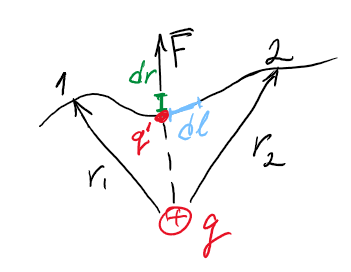
\includegraphics[width=6cm]{physics1/images/physics1_2024_11_25_1}
    \end{wrapfigure}

    Со стороны заряд $q$ на заряд $q^\prime$ действует сила $F$. Заряд $q^\prime$ движется по траектории, работа силы Кулона равна:

    $A = \int \vec{F}d\vec{l} = \int F dr = \int_{r_1}^{r_2} \frac{kqq^\prime}{r^2} dr$ \hfill $dr = dl \cos\alpha$

    $A = -\frac{kqq^\prime}{r} \Big|_{r_1}^{r_2} = \frac{kqq^\prime}{r_1} - \frac{kqq^\prime}{r_2} = W_1 - W_2$

    $A = \int_1^2 q^\prime \vec{E} d\vec{l} = q^\prime \int_1^2 \vec{E}d\vec{l}$

    Из этого выходит, что работа по замкнутому контуру равна нулю: $\oint \vec{E}d\vec{l} = 0$ - теорема о циркуляции
\end{minipage}

Теорема о циркуляции является вторым рассмотренным нами уравнением Максвелла

Из теоремы о циркуляции следует то, что силовые линии электрического поля не могут быть замкнутыми, а линии
однородного поля расположенны на одинаковом расстоянии друг от друга и параллельны друг другу

Теорема о циркуляции существует и в дифференциальной форме форме; 
по определению ротора $\math{rot} \vec{E} = \lim_{\Delta S \to 0} \frac{\oint \vec{E}d\vec{l}}{\Delta S}$:

\[\mathrm{rot} \vec{E} = 0\]

$A = W_1 - W_2 = q\varphi_1 - q\varphi_2 = q(\varphi_1 - \varphi_2) \hfill W = q \varphi$

Потенциал точки поля численно равен работе по перемещению точечного положительного заряда из бесконечности
в данную точку поля

$A = q(\varphi - \varphi_\infty) = q\varphi \Longrightarrow \varphi = \frac{A}{q}$

Потенциал на бесконечности равен 0: $\varphi_\infty = 0$

$\int_1^2 \vec{E} d\vec{l} = \varphi_1 - \varphi_2$

$\vec{E}d\vec{l} = E_l dl = -d\varphi$

$\vec{E} = -(\frac{\partial \varphi}{\partial x}\vec{i} + \frac{\partial \varphi}{\partial y}\vec{j} + \frac{\partial \varphi}{\partial z}\vec{k}) = -\mathrm{grad} \varphi = -\vec{\nabla} \varphi$

Потенциал измеряется в вольтах

Из этого можно получить данные преобразования:

$\mathrm{div} \vec{E} = \frac{\rho}{\varepsilon_0}$

$\vec{E} = -\mathrm{grad} \varphi$

$\mathrm{div}(-\mathrm{grad} \varphi) = -\Delta \varphi = \frac{\rho}{\varepsilon_0}$ - и получить уравнение Пуассона

$\varphi_1 - \varphi_2 = \int_1^2 \vec{E}d\vec{l} = El\cos\alpha$

В конденсаторе $E = \frac{\varphi_1 - \varphi_2}{d} = \frac{U}{d}$

\begin{minipage}{\textwidth}
    \begin{wrapfigure}{r}{0pt}
        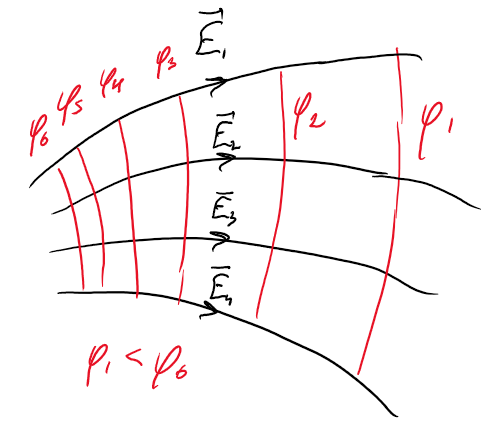
\includegraphics[width=6cm]{physics1/images/physics1_2024_11_25_2}
    \end{wrapfigure}
    Также электрическое поле изображают в виде эквипотенциальных поверхностей

    Эквипотенциальные поверхности проще линий напряженности тем, что они скалярные величины
\end{minipage}

\ExN{1} Точечный заряд

$\varphi_1 - \varphi_\infty = \int_r^\infty \vec{E}d\vec{l} = \int_r^\infty \frac{kq}{r^2} dr = -\frac{kq}{r} \Big|_r^\infty = \frac{kq}{r}$

\ExN{2} Линия или цилиндр

$\varphi_1 - \varphi_2 = \int_{r_1}^{r_2} \vec{E}d\vec{l} = \int_{r_1}^{r_2} \frac{2k\tau}{r} dl = 2k\tau \ln\frac{r_2}{r_1}$

Для линии, к сожалению, мы не можем найти потенциал в точке на бесконечности

\ExN{3} Сфера

Внутри сферы:

$\varphi_0 - \varphi_R = \int_0^R Edl = 0 \Longrightarrow \varphi_0 = \varphi_R$

Снаружи сферы:

$\varphi_r = \varphi_r - \varphi_\infty = \int_r^\infty \frac{kq}{r^2} dr = \frac{kq}{r}$

\begin{center}
    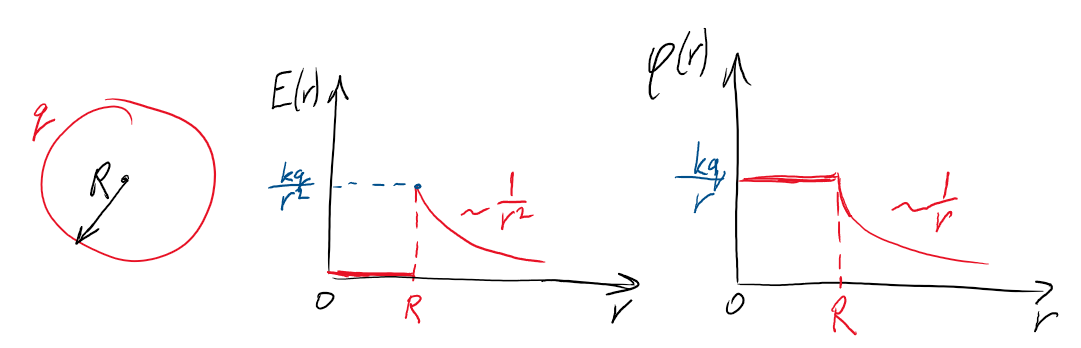
\includegraphics[width=0.9\textwidth]{physics1/images/physics1_2024_11_25_3}
\end{center}

\ExN{4} Шар

Снаружи шара:

$\varphi_r - \varphi_\infty = \int_r^\infty \frac{kq}{r^2} dr = \frac{kq}{r}$

Внутри шара:

$E = \frac{kqr}{R^2}$

$\varphi_0 - \varphi_R = \int_0^R \frac{kqr}{R^3} dr = \frac{kqr^2}{2R^3} \Big|_0^R = \frac{kq}{2R}$

$\varphi_0 = \varphi_R + \frac{kq}{2R} = \frac{kq}{R} \cdot \frac{3}{2}$

\begin{center}
    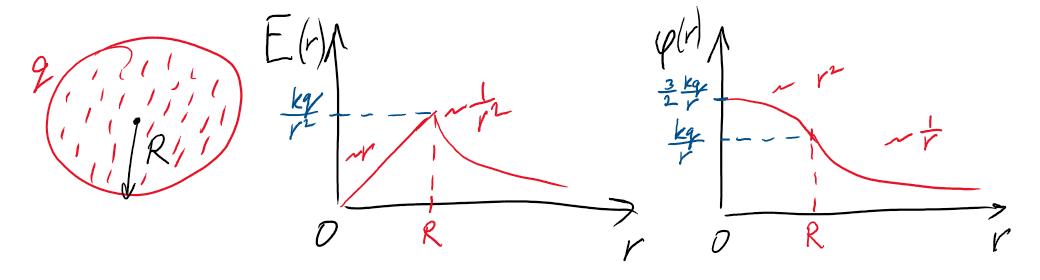
\includegraphics[width=0.9\textwidth]{physics1/images/physics1_2024_11_25_4}
\end{center}

\Nota Если шар сделан из диэлектрика, то не забываем про диэлектрическую проницаемость

\ExN{5} Распределение заряда 

\begin{center}
    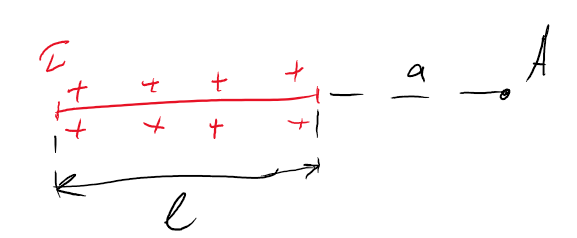
\includegraphics[width=0.5\textwidth]{physics1/images/physics1_2024_11_25_5}
\end{center}

$\varphi = \int d\varphi = \int \frac{kdq}{r} = \int_a^{a + l} \frac{k\tau dr}{r} = k\tau \ln\frac{a + l}{a}$

\mediumvspace

Принцип суперпозиции для потенциала:

\[\varphi = \varphi_1 + \varphi_2 + \dots + \varphi_n\]





